\subsection{SoC 设计}
在 SOC 顶层实例化了我们的 CPU ，向 SoC 提供单路 32 位 AXI 主接口和 8 路外部中断输入。

\begin{figure}[H]
  \centering
  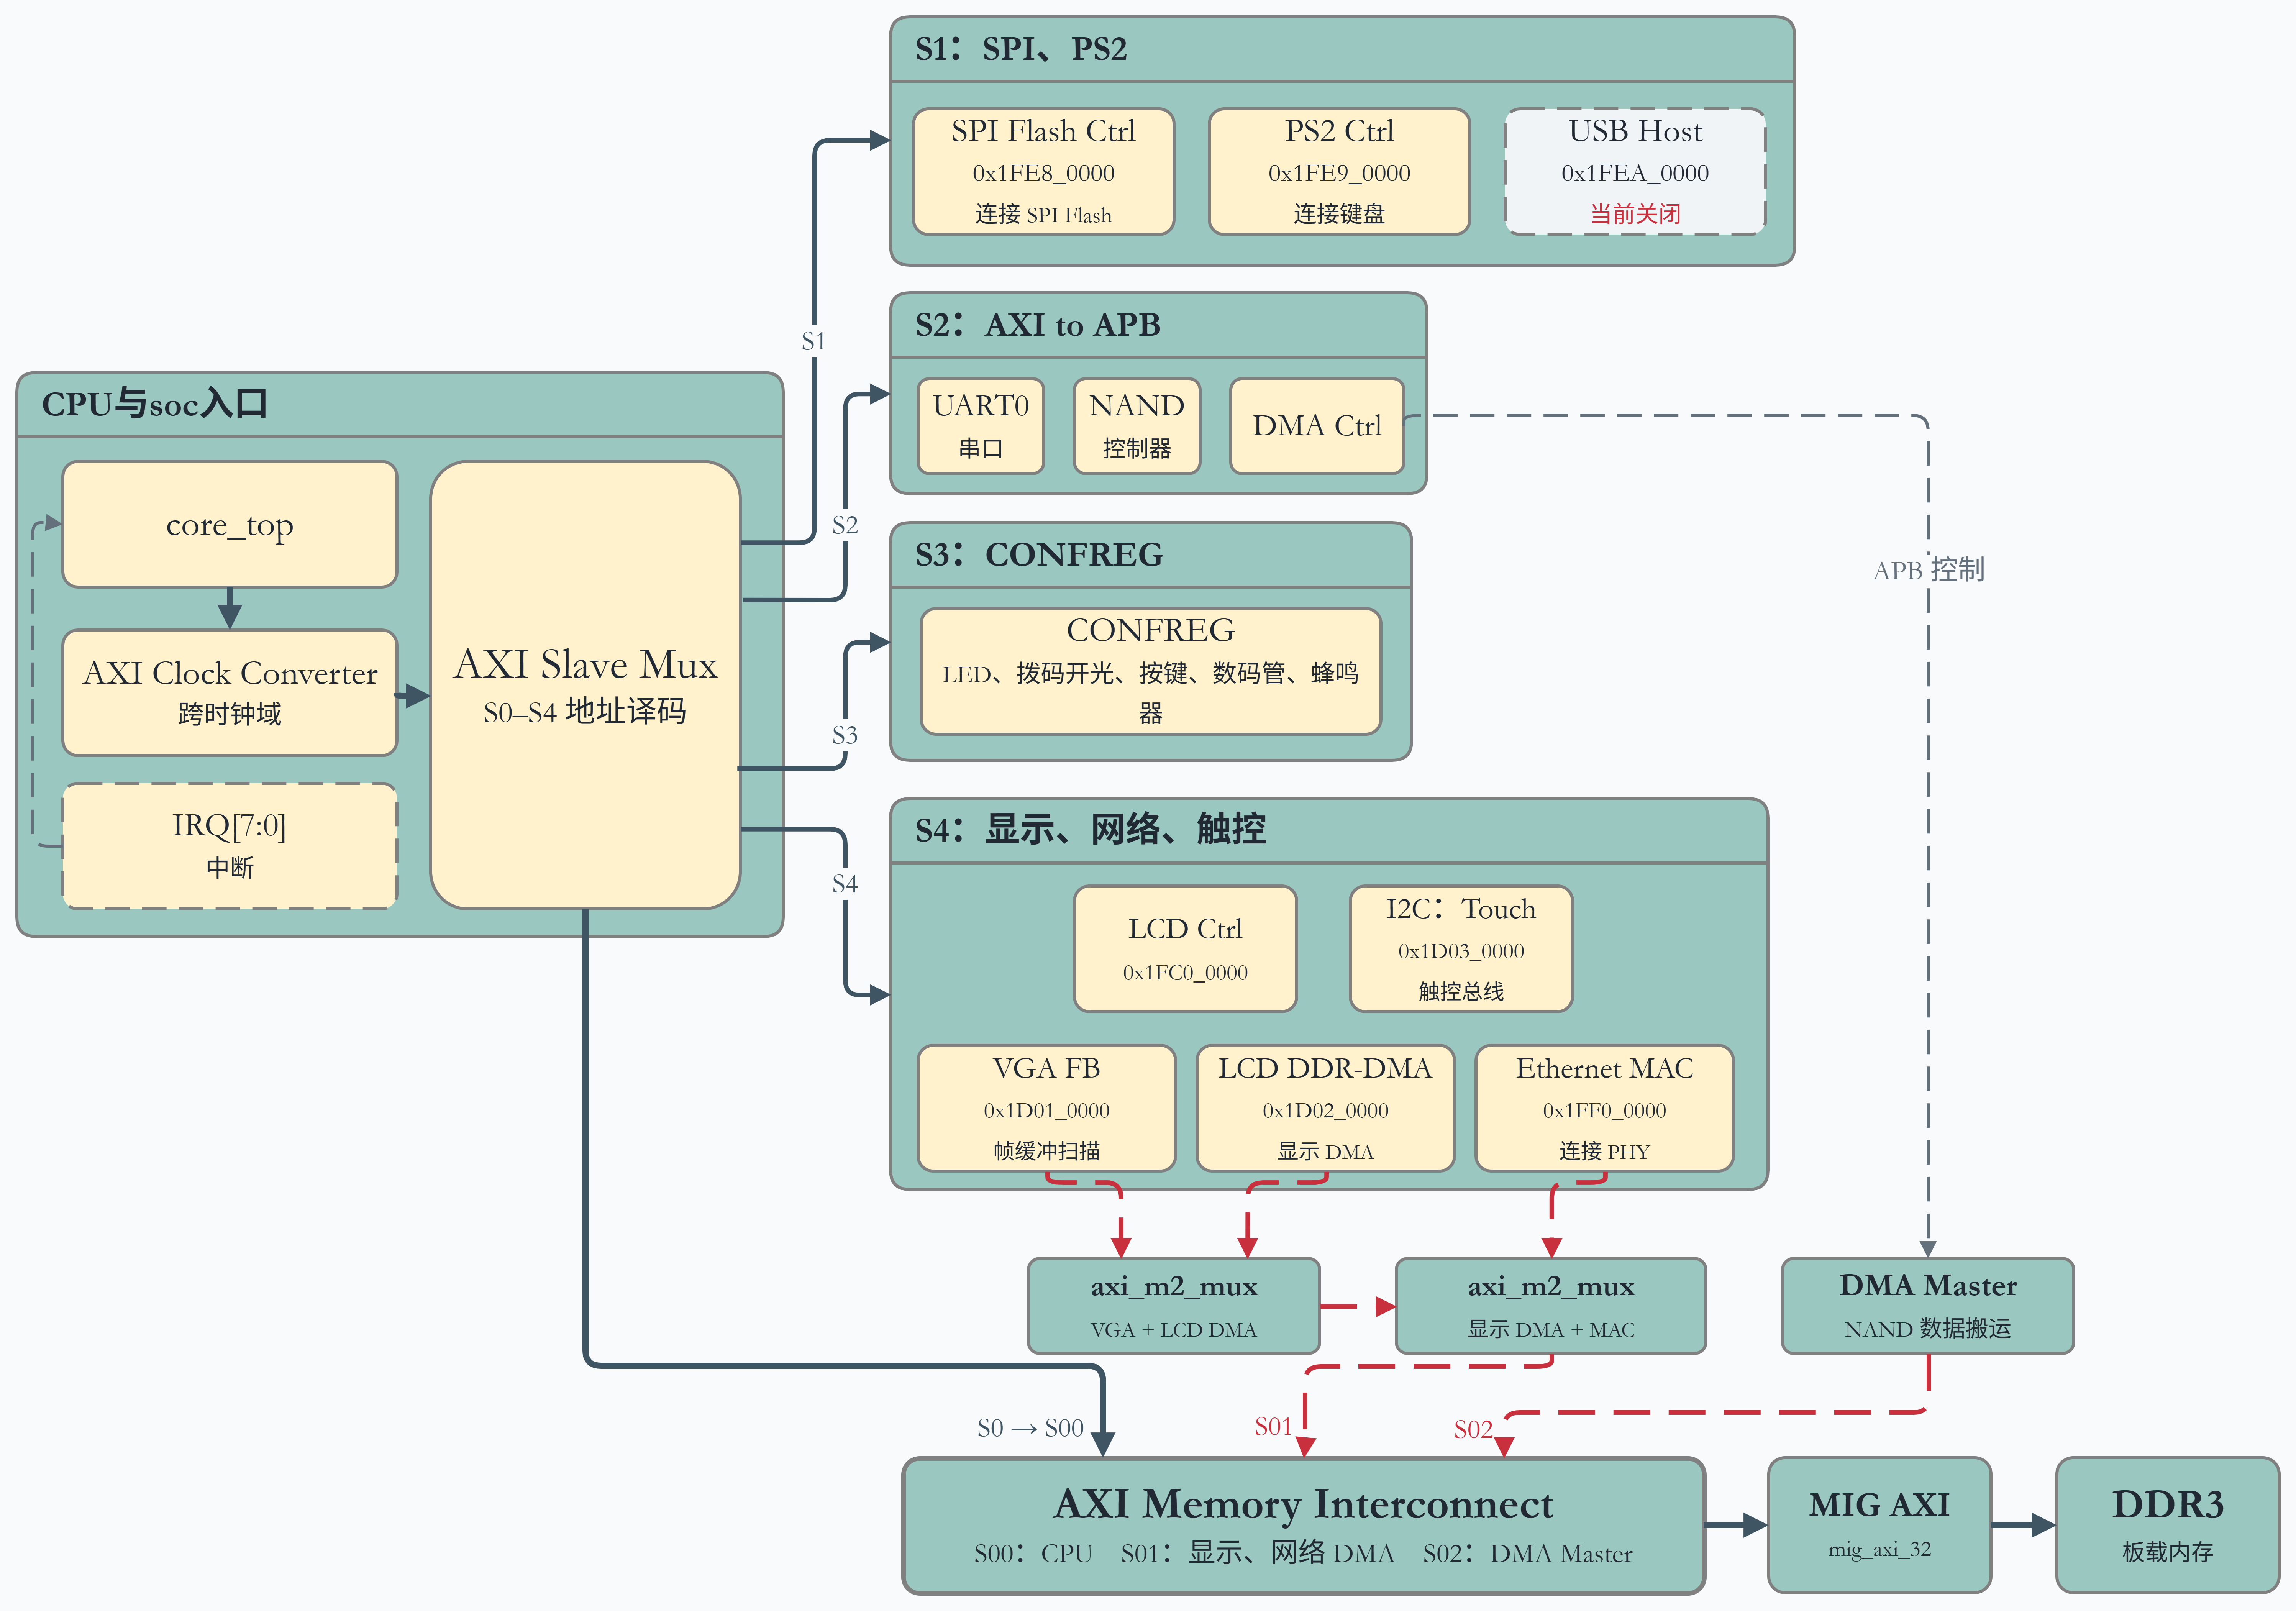
\includegraphics[width=0.95\textwidth]{figure/soc.png}
  \caption{soc架构图}
  \label{fig:soc}
\end{figure}

\subsubsection{互连、时钟与复位}

CPU AXI 经 AXI Clock Converter 进入 uncore 域，再由地址译码和 AXI/APB 互连分发至 DDR3、CONFREG 与各外设。DDR3 前端使用多主口互连，除 CPU 外，还承载 VGA/LCD/以太网 DMA 和 NAND/通用 DMA 流量。

\begin{table}[H]
\centering
\caption{SoC 主要时钟}
\label{tab:soc_clock}
\small
\begin{tabular}{lll}
\toprule
时钟 & 频率 & 用途 \\
\midrule
板级输入 & 100\,MHz & PLL 与时钟管理输入 \\
CPU & 60\,MHz & 处理器核与 CPU 侧 AXI \\
uncore & 60\,MHz & 外设、APB 与 SoC 主互连 \\
MIG 参考 & 200\,MHz & DDR3 PHY 参考 \\
MIG UI / DDR AXI & 100\,MHz & DDR3 用户接口 \\
VGA 像素 & 25\,MHz & 640$\times$480@60\,Hz 输出 \\
MII RX/TX 接口 & 25\,MHz & 以太网收发时钟 \\
\bottomrule
\end{tabular}
\end{table}

CPU 复位采用异步拉低、同步释放；DDR 相关逻辑还等待 PLL 锁定、MIG 校准完成和 UI 复位释放。PLL 失锁或 uncore 复位会重新复位 CPU 与跨时钟域桥，避免总线两侧进入不一致状态。

\subsubsection{地址分配}

\begin{table}[H]
\centering
\caption{SoC 主要物理地址映射}
\label{tab:addr}
\scriptsize
\begin{tabularx}{\textwidth}{>{\ttfamily}p{3.4cm}>{\raggedright\arraybackslash}p{3.2cm}X}
\toprule
地址 & 模块 & 说明 \\
\midrule
0x00000000--0x07FFFFFF & DDR3 & 128\,MiB 系统内存 \\
0x0A000000 & VGA Framebuffer & RGB565 默认 DMA 地址；经 MIG 低 27 位寻址别名至 DDR 0x02000000 \\
0x1C000000--0x1C0FFFFF & SPI Flash Window & 启动镜像和存储器访问窗口 \\
0x1D010000 & VGA Controller & DDR 帧缓冲显示控制 \\
0x1D020000 & LCD DMA & LCD 独立 DDR 读取通道 \\
0x1D030000 & I2C Master & 通用 I2C 与触摸共享总线 \\
0x1FC00000 区域 & LCD Controller & 8080 接口 LCD 控制，常用寄存器位于 0x1FC0C000 \\
0x1FD00000 区域 & CONFREG & GPIO、定时器、LED、数码管、按键、蜂鸣器与 DMA 控制 \\
0x1FE001E0 & UART & 16550 串口数据与控制端口 \\
0x1FE70000 区域 & NAND & NAND 控制器，Linux 节点使用 0x1FE78000 \\
0x1FE80000 & SPI Controller & SPI Flash 控制寄存器 \\
0x1FE90000 & PS/2 & 键盘/鼠标控制器 \\
0x1FEA0000 & USB Host & 保留窗口，当前工程未启用 \\
0x1FF00000 & Ethernet MAC & MII 10/100M MAC 与 DMA \\
\bottomrule
\end{tabularx}
\end{table}

地址译码未匹配的访问会落入 DDR 路径，而 MIG 仅使用低 27 位地址。软件将规范 DDR 可用范围限制为 128\,MiB，避免高地址别名。

\subsubsection{外设与中断}

我们的 SOC 集成 UART、SPI、NAND、PS/2、GPIO、定时器、LED、数码管、蜂鸣器、VGA、8080 LCD、I2C 与 MII Ethernet。USB Host RTL 和管脚接口仍保留，但配置宏关闭；EJTAG 与调试 UART 也只作为保留接口，不作为当前已完成的调试功能。

\begin{table}[H]
\centering
\caption{CPU 外部中断映射}
\label{tab:interrupt}
\small
\begin{tabular}{cl}
\toprule
CPU 中断位 & 中断源 \\
\midrule
0 & Ethernet MAC \\
1 & UART \\
2 & SPI \\
3 & NAND \\
4 & DMA \\
5 & PS/2 \\
6 & 保留；启用 USB Host 时可连接 USB \\
7 & 保留 \\
\bottomrule
\end{tabular}
\end{table}

所有 uncore 外设中断在送入 CPU 前经过两级同步。VGA 使用 640$\times$480@60\,Hz、RGB565 DDR 帧缓冲；LCD 使用 16 位 8080 接口并可由独立 DMA 从 DDR 读取图像。
